\documentclass{beamer}

\usepackage[frenchb]{babel}
\usepackage[T1]{fontenc}
\usepackage[utf8]{inputenc}
\usepackage{amsmath}


\usetheme{Frankfurt}

\title{HMIN 320 - Projet}
\author{Noé LE PHILIPPE - Samuel BRICAS}
\institute{Université de Montpellier}
\date{\today}
% \logo{\includegraphics[height=10mm]{images/logo.png}}

\addtobeamertemplate{navigation symbols}{}{%
  \usebeamerfont{footline}%
  \usebeamercolor[fg]{footline}%
  \hspace{1em}%
  \insertframenumber/\inserttotalframenumber
}

\AtBeginSection[]
{
  \begin{frame}
    \frametitle{Sommaire}
    \tableofcontents[currentsection, hideothersubsections]
  \end{frame} 
}

\begin{document}

\begin{frame}
  \titlepage
\end{frame}

\section{Présentation du sujet}
\subsection{Description du sujet}
\begin{frame}
  \frametitle{Présentation du sujet}
  \begin{block}{Le jeu}
    Un ``pierre-feuille-ciseaux'' contre l'ordinateur
  \end{block}
  \begin{block}{Les joueurs}
    Monojoueur, l'adversaire est le CPU
  \end{block}
  \begin{block}{L'interface}
    Le jeu se joue à la webcam
  \end{block}
\end{frame}
\subsection{Technologies}
\begin{frame}
  \frametitle{Technologies utilisées}
  
\includegraphics[scale=0.8]{./opencv_logo.png}
  
\includegraphics[scale=0.2]{./cpp.jpeg}
\end{frame}
\subsection{Un changement de projet ?}
\begin{frame}
  \begin{center}
    \frametitle{Un changement de projet ?}
    
\includegraphics[scale=0.5]{./cher.png}
  \end{center}
\end{frame}
\subsection{Pourquoi OpenCV ?}
\begin{frame}
  \frametitle{Pourquoi OpenCV ?}
  \begin{block}{}
    Apprentissage d'un nouvel outil
  \end{block}
  \begin{block}{}
    Pas une simple utilisation d'API de devices existants
  \end{block}
\end{frame}
\subsection{Principes du jeu}
\begin{frame}
  \frametitle{Principes du jeu}
  L'ordinateur détecte la main du joueur, le coup joué, et joue en fonction
\end{frame}
\section{La detection}
\subsection{Extraction de la main}
\begin{frame}
  \frametitle{Extraction de la main}
  \begin{block}{}
    Construction du background
  \end{block}
  \begin{block}{}
    Soustraction du background et de la frame courante
  \end{block}
  \begin{block}{}
    Extraction des contours
  \end{block}
  \begin{block}{}
    Sauvegarde du plus grand contours avec la plus faible variance : c'est la main
  \end{block}
\end{frame}
\begin{frame}
  \frametitle{Extraction de la main}
  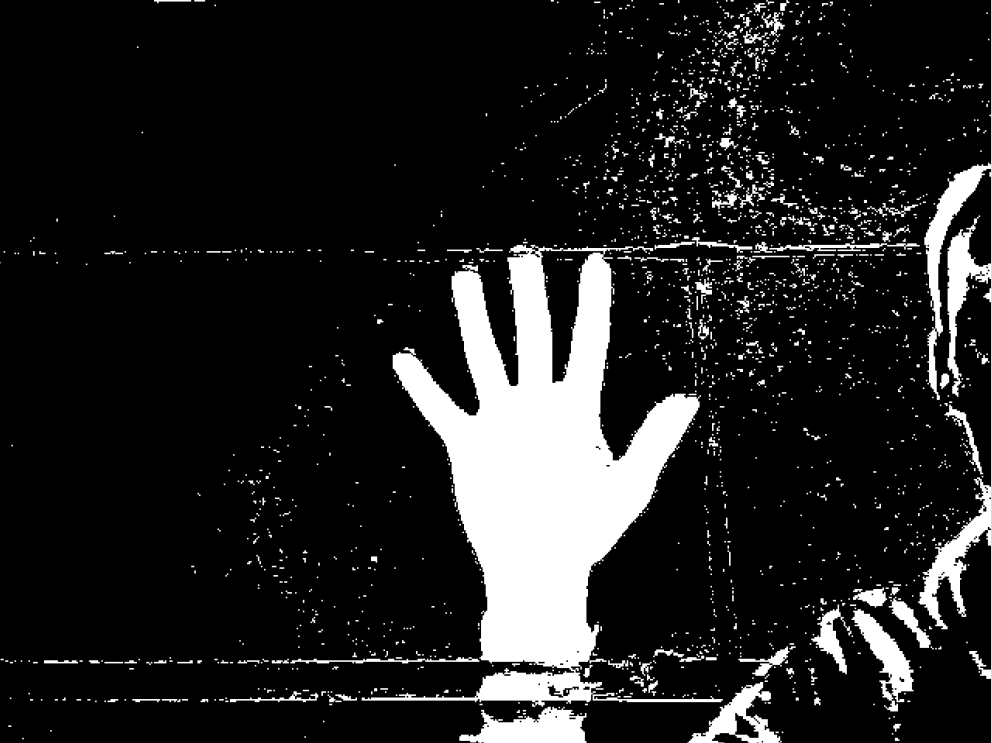
\includegraphics[scale=0.3]{background.png}
\end{frame}
\begin{frame}
  \frametitle{Extraction de la main}
  
\includegraphics[scale=0.3]{background_hand.png}
\end{frame}
\subsection{Analyse de la main}
\begin{frame}
  \frametitle{Analyse de la main}
  \begin{block}{}
    Construction de l'enveloppe convexe
  \end{block}
  \begin{block}{}
    Calcul des défauts de convexité
  \end{block}
  \begin{block}{}
    Filtrage des défauts de convexité
  \end{block}
  \begin{block}{}
    Extraction des doigts
  \end{block}
\end{frame}
\begin{frame}
\begin{figure}
   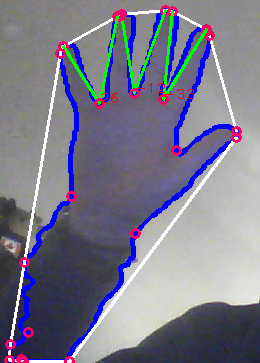
\includegraphics[width=0.475\textwidth]{./unfiltered.png}
   \hfill
   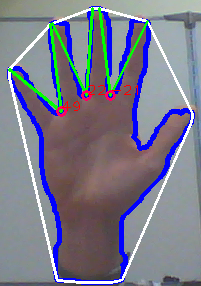
\includegraphics[width=0.475\textwidth]{./filtered.png}
\end{figure}
\end{frame}
\end{document}
